\section{Technische Grundlagen}
\subsection{DCF77}
TODO

\subsection{LED Matrix}
Unter LED Matrix versteht man die Ansteurung von LEDs in Zeilen und Spalten. Dabei werden alle Anoden zu Spalten und alle Kathoden zu Zeilen
verbunden. \footnote{Es kann natürlich auch die Kathode für Spalten und die
Anode für Spalten verwendet werden.} Im Vergleich zu einer einzelansteurung
bietet die LED MAatrix den großen Vorteil das bei einer Matrix $N$ Spalten
und $M$ Zeilen nur $N+M$ statt $N*M$ Leitungen verwendet werden.

\begin{wrapfigure}{r}{0.45\textwidth}
  \vspace{-25pt}
  \begin{center}
    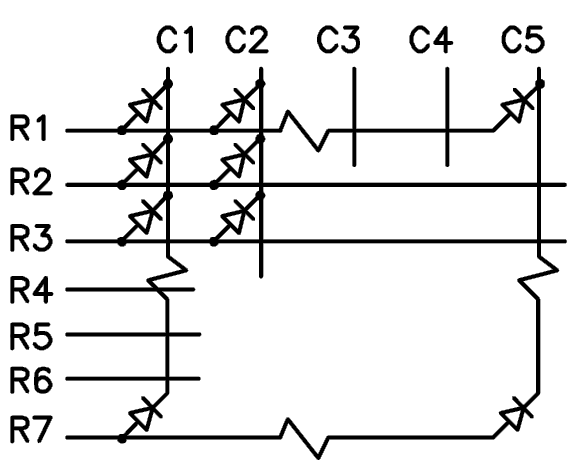
\includegraphics[width=0.42\textwidth]{skizzen/led_matrix_5x7.png}
  \end{center}
  \vspace{-20pt}
  \captionof{figure}{5x7 LED Matrix}
\end{wrapfigure}

Die LED Matrix
wird dann Zeilenweise oder Spatenweise im Multiplexbetrieb angesteuert. Das bedeutet nacheinander wird eine der Spalten mit GND versorgt und die anderen Spalten sind unbeschalten (keine Verbindung zu GND). Nun können in dieser Spalte durch anlegen von Spannung an den entsprechenden Zeilen LEDs angeschaltet werden. 
Dieser Vorgang wird für alle Spalten durchgeführt, das bedeutet es leuchten zu
einem bestimmten Zeitpunkt immer nur die LEDs einer Spalte. Durch das schnelle
umschalten zwischen den Spalten und die Trägheit des menschlichen Auge entsteht
die Illusion, dass auf der kompletten LED Matrix etwas LEDs aktiviert sind.
Als Nachteil aus dieser Beschaltung ergibt sich die veringerte Helligkeit, da
die LEDs bei $N$ Spalten nur noch $1/N$ der Zeit leuchten können.

Der Helligkeitsverlust kann durch höheren Stromfluss zum Teil kompensiert
werden. Dass bedeutet bei $N$ Spalten werden die LEDs mit einem Pulsstrom von
$N*Nennstrom$ betrieben. Durch die Dunkelphasen kann das aktive Substrat
zwischen den Pulsen ausreichend abkühlen. Generell kann dies bis zum ca.
zehnfachen Nennstrom (200mA bei einer gewöhnlichen 20mA LED) durchgeführt
werden.\footnote{http://www.mikrocontroller.net/articles/LED-Matrix}




\subsection{Pulsweitenmodulation}\label{sec_pulsweitenmodulation}
TODO